\documentclass{article}
\usepackage{ctex}
\usepackage{amsmath}
\usepackage{hyperref}
\usepackage{fancyhdr}
\usepackage{fontspec}
\usepackage{graphicx}
\usepackage{subfigure}
\setmainfont[Mapping=tex-text]{KaiTi}

\topmargin=-0.45in
\evensidemargin=0in
\oddsidemargin=0in
\textwidth=6.5in
\textheight=9.0in
\headsep=0.25in
\linespread{1.1}



%配置区
\newcommand{\courseName}{模式识别}
\newcommand{\homeworkId}{\#3} %作业编号
\newcommand{\homeworkTitle}{作业\homeworkId}
\newcommand{\studentId}{201928014629008}%学号
\newcommand{\studentName}{牛李金梁}%姓名



\newcommand{\question}[1]{\section*{Question #1}}
\renewcommand{\part}[1]{\subsection*{(#1)}}



\pagestyle{fancy}
\lhead{\studentName}
\rhead{\courseName\homeworkTitle}
\cfoot{\thepage}

\title{
    \vspace{2in}
    \textmd{\textbf{\courseName}:\homeworkTitle}\\
    \vspace{0.1in}
    \large{\studentId}\\
    \large{\studentName}\\
    \vspace{3in}
}

\begin{document}


\maketitle
\date{}
\pagebreak

\section*{第一部分:计算与证明}

\question{1}
首先,对样本进行规范化增广。根据设定,样本$\pmb{x}$增加齐次坐标后$\pmb{y} = (\pmb{x}^T, 1)^T$,
之后将第二类样本$\pmb{y}$变为$-\pmb{y}$,便得到4个规范化增广样本:

第一类样本为$(1, 4, 1)^T$和$(2, 3, 1)^T$,第二类样本为$(-4, -1, -1)^T$和$(-3, -2, -1)^T$。

初始权向量为$\pmb{a} = (0, 1, 0)^T$,梯度更新步长$\eta_k = 1$,利用Batch Perceptron算法迭代:
\begin{itemize}
	\item [1)] 
	$\pmb{a} = (0, 1, 0)^T$,对于样本$(-4, -1, -1)^T$和$(-3, -2, -1)^T$,
	有$\pmb{a}^T\pmb{y} < 0$。对错分样本求和,$\sum\limits_{y \in Y}\boldsymbol{y} = (-7, -3, -2)^T$。
	由更新准则$\pmb{a}_2 = \pmb{a}_1 + \eta_k \sum\limits_{y \in Y}\pmb{y} = (-7, -2, -2)^T$。
	\item [2)]
	$\pmb{a} = (-7, -2, -2)^T$,对于样本$(1, 4, 1)^T$和$(2, 3, 1)^T$,
	有$\pmb{a}^T\pmb{y} < 0$。对错分样本求和,$\sum\limits_{y \in Y}\boldsymbol{y} = (3, 7, 2)^T$。
	由更新准则$\pmb{a}_3 = \pmb{a}_2 + \eta_k \sum\limits_{y \in Y}\pmb{y} = (-4, 5, 0)^T$。
	\item [3)]
	$\pmb{a} = (-4, 5, 0)^T$,对于所有样本有$\pmb{a}^T\pmb{y} > 0$。
	无错分样本。
\end{itemize}

所以线性判别函数$g(\pmb{y}) = \pmb{a}^T\pmb{y}$的权向量为$\pmb{a} = (-4, 5, 0)^T$。

\question{2}
根据one-vs-all的规则,本问题需设计一个线性机器,
将样本空间分为3个决策区域$R_1$,$R_2$,$R_3$,
分别对应决策为3个类别$\omega_1$,$\omega_2$,$\omega_3$。
\begin{itemize}
	\item[*] $R_1$和$R_2$的分界面$H_{12}$为
	$g_1(\pmb{x}) - g_2(\pmb{x}) = -2x_1 + 1 = 0$。
	\item[*] $R_1$和$R_3$的分界面$H_{13}$为
	$g_1(\pmb{x}) - g_3(\pmb{x}) = -x_1 + 2x_2 = 0$。
	\item[*] $R_2$和$R_3$的分界面$H_{23}$为
	$g_2(\pmb{x}) - g_3(\pmb{x}) = x_1 + 2x_2 -1 = 0$。
\end{itemize}

画出$H_{12}$、$H_{13}$、$H_{23}$3个分界面,
并根据决策规则确定$R_1$、$R_2$、$R_3$的位置,如图:

\begin{figure}[ht]
	\centering
	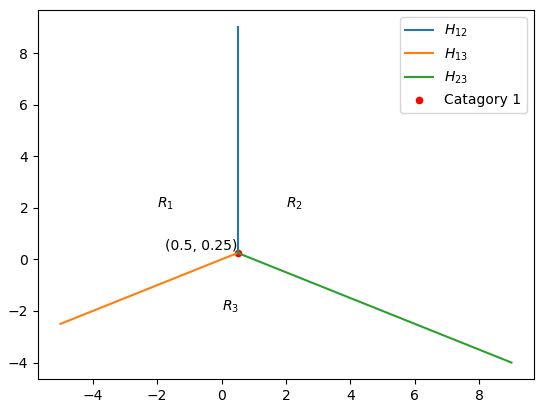
\includegraphics[width=0.5\textwidth]{Figure_1.png}
	\caption{决策区域示意图}
	\label{figl}
\end{figure}

可见,决策区域的分界面相交于$(0.5, 0.25)$,该问题不存在不确定区域。
同样地,使用该决策规则构造线性机器,实际上是将样本分类到判别函数最大
的那个类别中,因此除边界上的点外不会存在不确定区域。

\section*{第二部分:计算机编程}
环境为python3.7

依赖库:numpy、matplotlib

运行方式:直接在cmd中执行相应py文件

\question{1}
使用Batch perception算法训练判别函数,首先要对样本进行规范化增广,
然后利用这些样本训练线性判别函数。

具体的训练过程需要将每一步错分的点相加并乘以步长来修正权向量$\pmb{a}$,
如此迭代直至完全分开或修正值很小(以应对线性不可分的情况)。

实验中,取初始权向量$\pmb{a} = \pmb{0}$,$\eta = 1$,$\theta = 0.01$,
结果如下图:
\begin{figure}[ht]
	\centering
	\subfigure{
		\begin{minipage}[t]{0.45\linewidth}
			\centering
			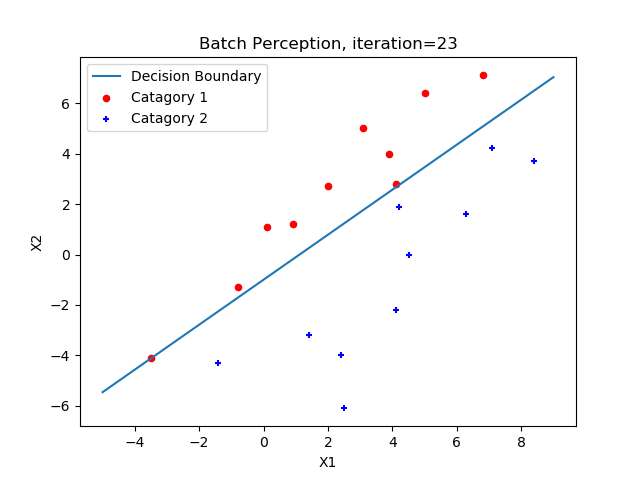
\includegraphics[width=3in]{Figure_2.png}
		\end{minipage}
	}
	\subfigure{
		\begin{minipage}[t]{0.45\linewidth}
			\centering
			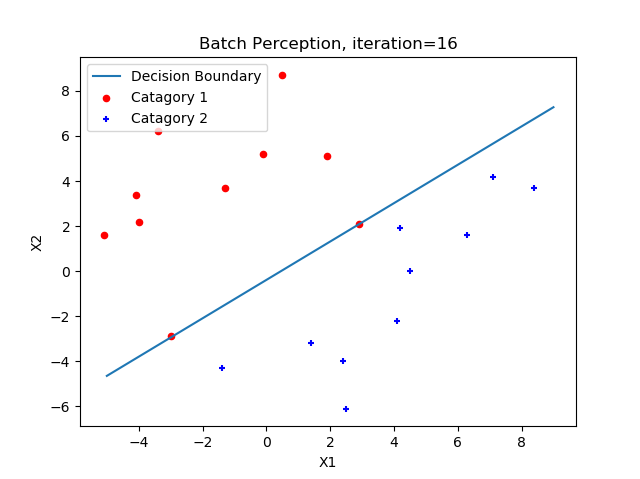
\includegraphics[width=3in]{Figure_3.png}
		\end{minipage}
	}
	\centering
	\caption{Batch perception算法结果}
	\label{figl}
\end{figure}

问题(a)中分类$\omega_1$和$\omega_2$的结果如左图所示,判别函数左上
判别为$\omega_1$,右下判别为$\omega_2$,收敛步数为23。

问题(b)中分类$\omega_3$和$\omega_2$的结果如右图所示,判别函数左上
判别为$\omega_3$,右下判别为$\omega_2$,收敛步数为16。

\question{2}
Ho-Kashyap算法通过最小化误差来优化$b$,并通过$a = Y^+ b$
计算对应的$a$,进而得到一组$a, b$使$Ya = b > 0$。 

搜索到最优解是比较困难的,需要设定最大迭代次数和收敛误差。
本程序设定步长为0.8,最大迭代次数为$2000$,收敛误差为$0.01$,
若所有样本的误差小于$b_{min}$(设定为0.001)或迭代$2000$次,则停止迭代。


$\omega_1$和$\omega_3$的分类结果如下图中左图所示,
决策面左上方为$\omega_3$,右下方为$\omega_1$。
可以看到有2个分类错误点,并且输出了No solution found,
说明该问题是线性不可分的。

$\omega_2$和$\omega_4$的分类结果如下图中右图所示,
决策面左下方为$\omega_4$,右上方为$\omega_2$。
可以看出该问题是线性可分的,迭代次数为899。
\begin{figure}[ht]
	\centering
	\subfigure{
		\begin{minipage}[t]{0.45\linewidth}
			\centering
			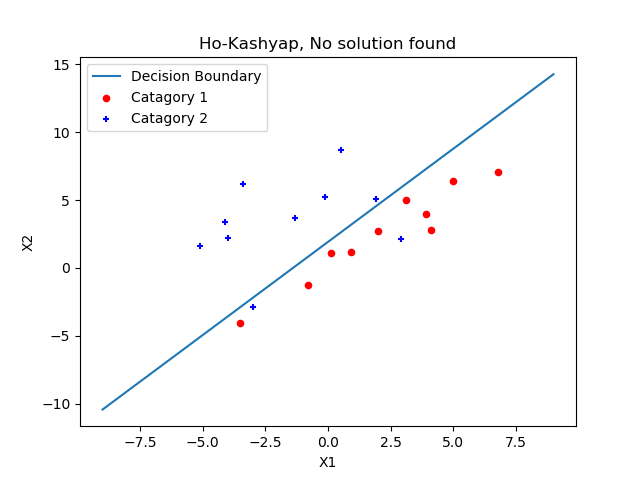
\includegraphics[width=3in]{Figure_4.png}
		\end{minipage}
	}
	\subfigure{
		\begin{minipage}[t]{0.45\linewidth}
			\centering
			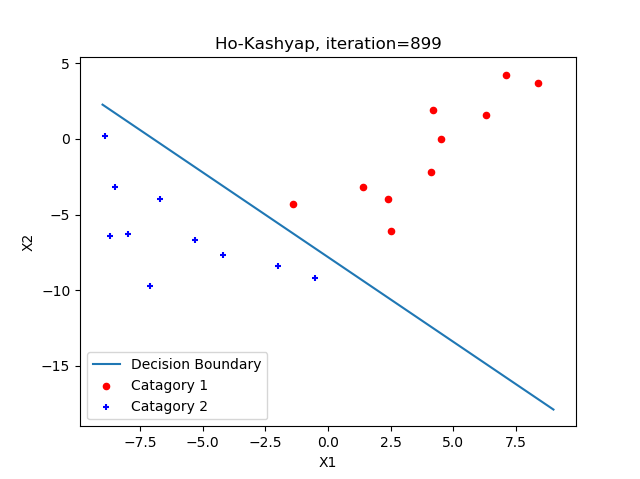
\includegraphics[width=3in]{Figure_5.png}
		\end{minipage}
	}
	\centering
	\caption{Ho-Kashyap算法结果}
	\label{figl}
\end{figure}

\question{3}
使用MSE多类扩展方法对4个类别进行分类。

具体的算法实现中,主要是要构造$\pmb{Y}$,并利用
${\hat W = {(\hat X{\hat X^T} + \lambda I)^{ - 1}}\hat X{Y^T}}$
来计算$\hat W$确定分类区域,程序中设定$\lambda = 0.01$。

根据决策规则$x \in \omega_i, g_i(x) = \max  g_j(x), j = 1, \dots, 4$
可以绘制出决策区域(本程序直接利用点采样确定了决策区域,而非计算线性判别函数),

\begin{figure}[ht]
	\centering
	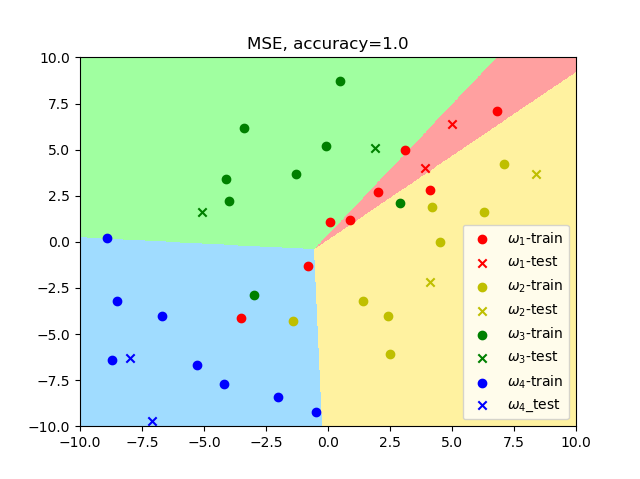
\includegraphics[width=0.5\textwidth]{Figure_6.png}
	\caption{决策区域示意图}
	\label{figl}
\end{figure}

图中红色为$\omega_1$决策区域,
黄色为$\omega_2$决策区域,绿色为$\omega_3$决策区域,
蓝色为$\omega_4$决策区域。
并以实心圆标记训练样本,x标记测试样本,
通过统计可以得到测试样本的分类正确率为100\%。
\end{document}